%Author - Aayush Goyal
%Date - 1/4/20
%Licence - GNU GPL
\begin{enumerate}[label=\thesection.\arabic*.,ref=\thesection.\theenumi]
\numberwithin{equation}{enumi} 
\item
%\begin{flushleft}
\textsf{ For an LTI system, the Bode plot for its gain is as illustrated in the Fig.2.1 The number of system poles $N_{p}$ and number of system zeros $N_{z}$ in the frequency range 1 Hz $\leq$ f $\leq$ $10^{7}$ Hz is}
%\end{flushleft}

\begin{figure}[htp]
    \centering
    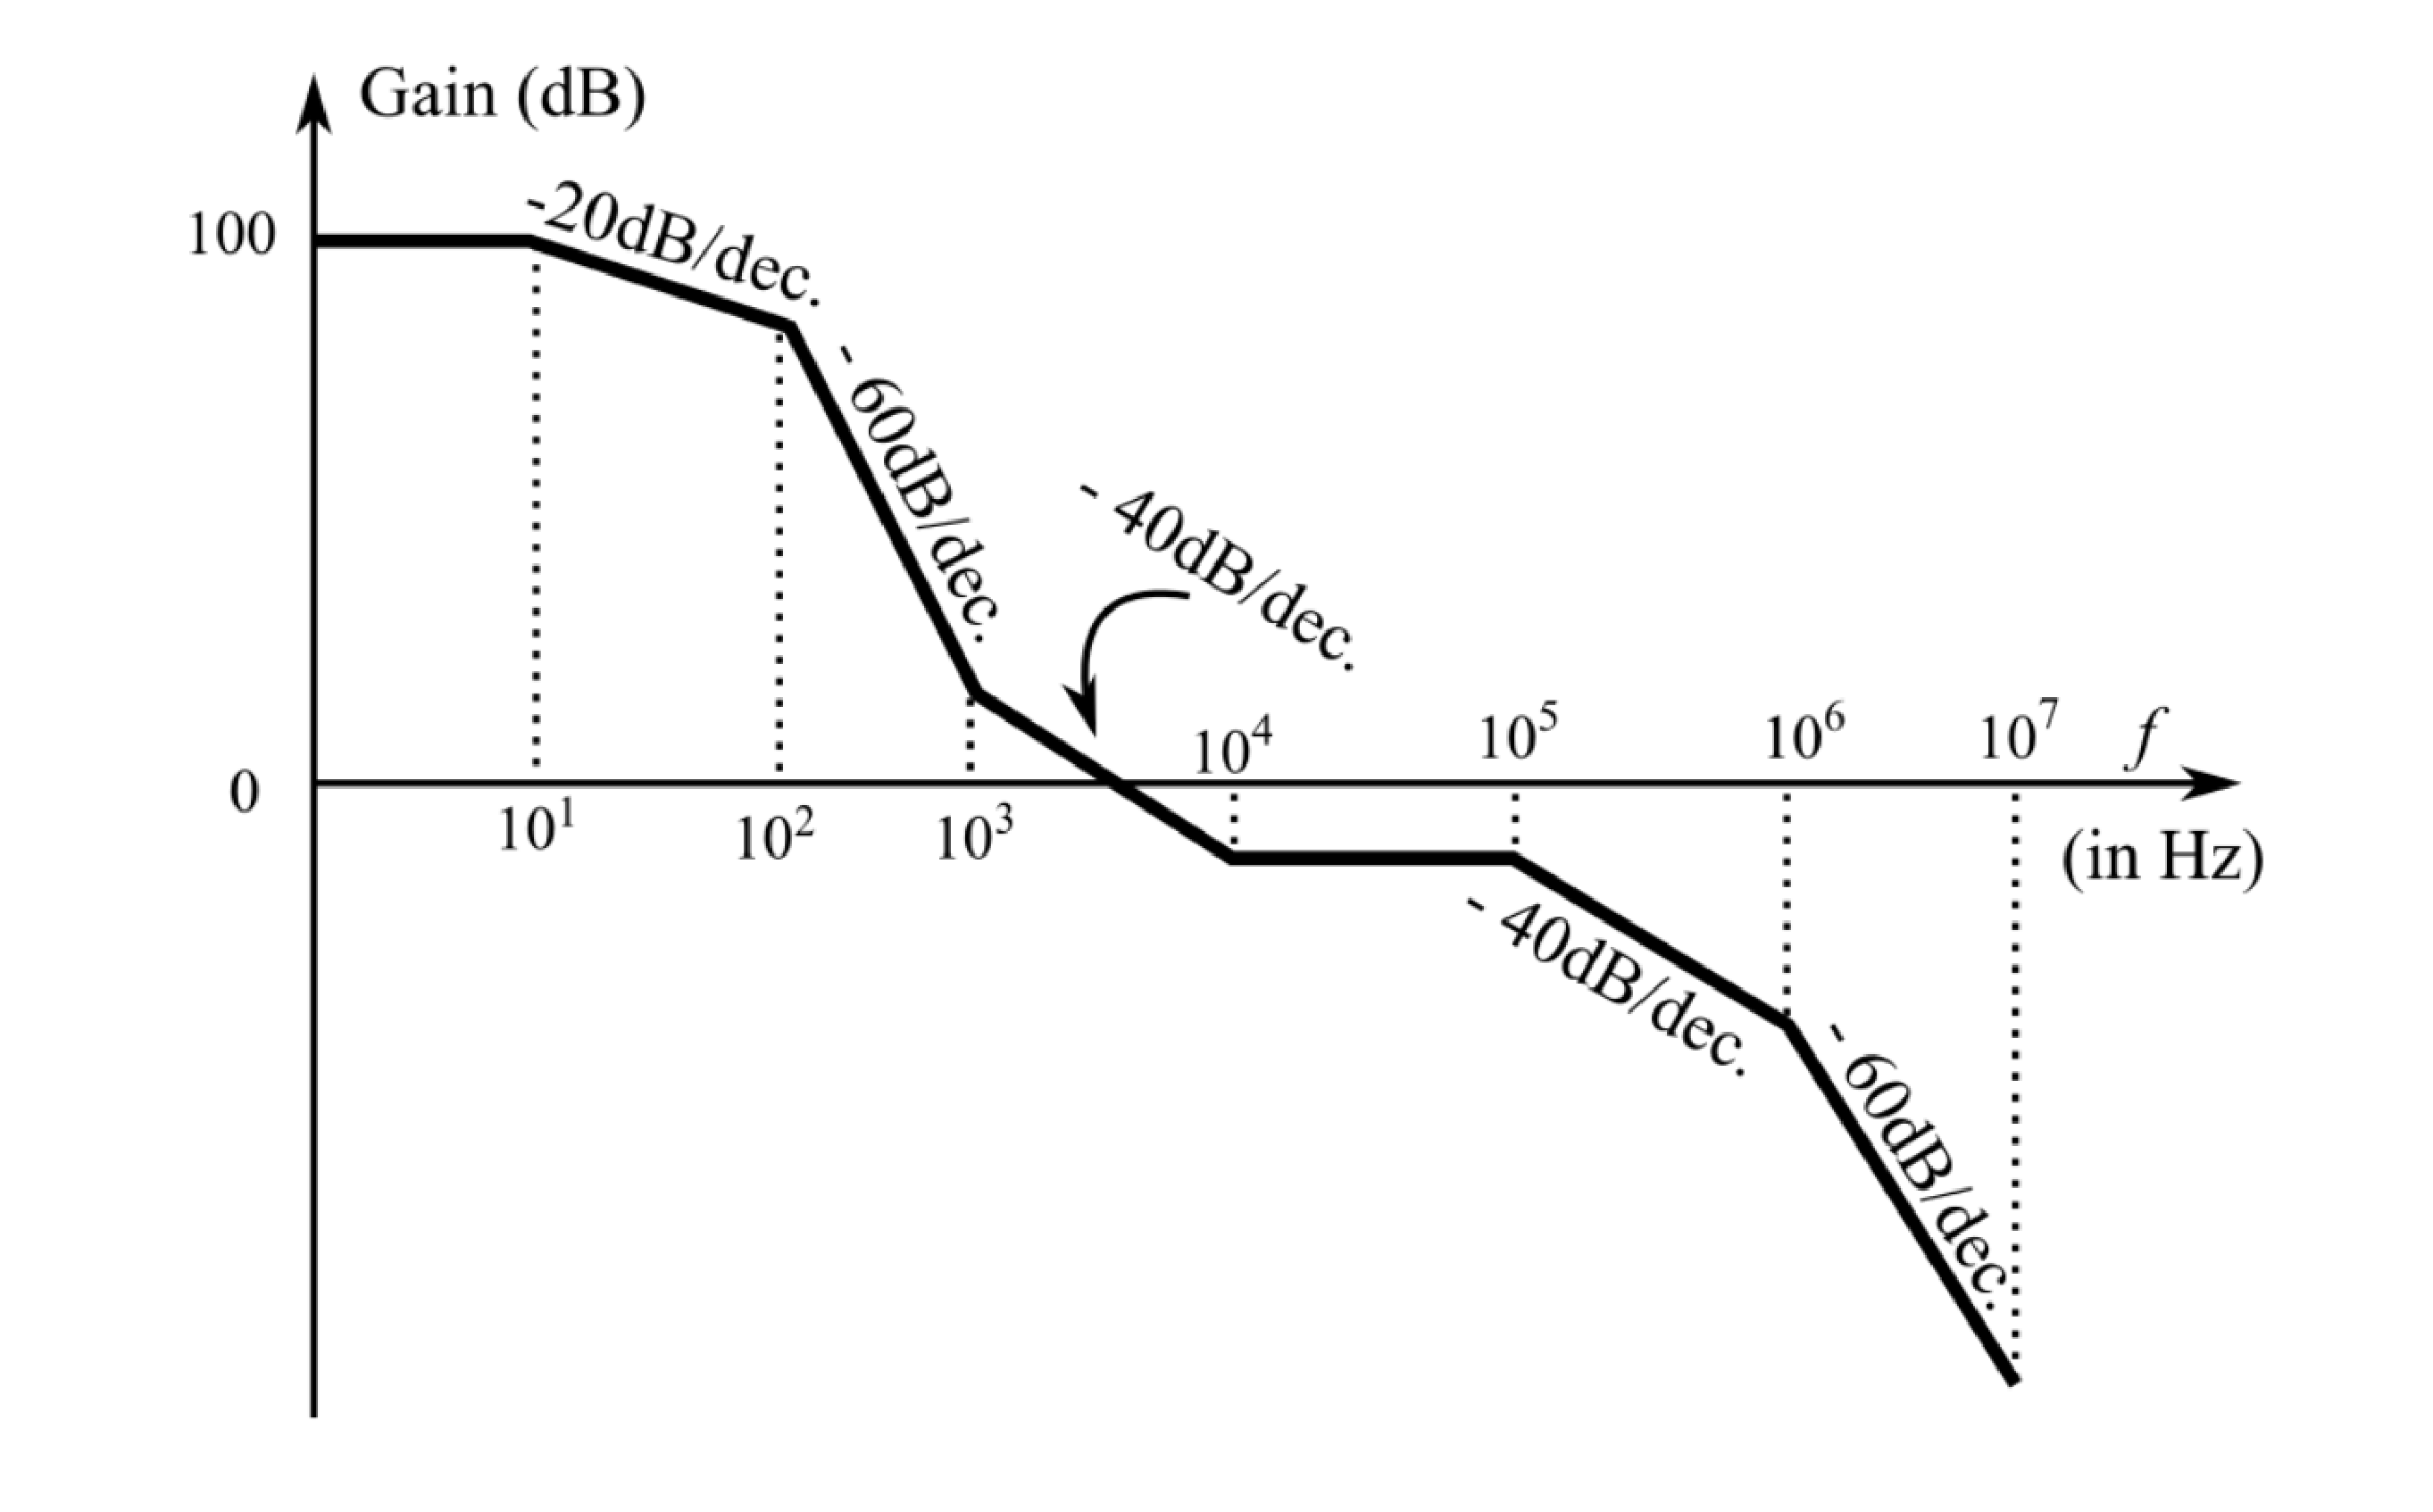
\includegraphics[width=\columnwidth]{./figs/ee18btech11001.eps}
    \caption{}
    \label{fig:galaxy}
\end{figure}

\solution 
\textsf{Let us consider a generalized transfer gain}
\\
\begin{align}
H(s) = k \dfrac{(s-z_{1})(s-z_{2})...(s-z_{m-1})(s-z_{m})}{(s-p_{1})(s-p_{2})....(s-p_{n-1})(s-p_{n})}
\end{align}
\begin{multline}
Gain = 20\log\abs{H(s)} = 20\log \abs{k} + 20\log \abs{s-z_{1}} 
    \\
    + 20\log \abs{s-z_{2}} + \dots + 20\log \abs{s-z_{m}} - 20\log \abs{s-p_{1}} 
    \\
    - 20\log \abs{s-p_{2}} - \dots - 20\log \abs{s-z_{n}} 
\end{multline}



Let us consider a $ 20\log \abs{s-z_{1}} $
\\
Let $s = j\omega$
\\

\begin{align}
	20\log \abs{s-z_{1}} = 20\log \abs{\sqrt{\omega^{2} + z_{1}^{2}}} 
\end{align}

Based on log scale plot approximations,to the 
left of $z_{1} \hspace{5pt} \omega << z_{1} $ and towards right  $ \omega >> z_{1} $
\\ \\
For $\omega < z_{1}$

\begin{align}
	20\log \abs{s-z_{1}} = 20\log \abs{\sqrt{\omega^{2} + z_{1}^{2}}} 
	&= 20 \log \abs{z_{1}} 
	&= constant 
\end{align}  
i.e. $Slope = 0$
\\
For $\omega > z_{1}$

\begin{align}
	20\log \abs{s-z_{1}} = 20\log \abs{\sqrt{\omega^{2} + z_{1}^{2}}} = 20 \log \abs{\omega} 
\end{align}

i.e $Slope = 20 $
\\
\textbf{When a zero is encountered the slope always increases by 20 dB/decade}
\\
\\
Doing similar analysis for $ - 20\log \abs{s-p_{1}} $  We conclude
\\
\textbf{When a pole is encountered the slope always decreases by 20 dB/decade}
\\

\begin{align}
Slope = \dfrac{d(20\log H(f))}{df}
\end{align}

\begin{align}
 Slope = 
 \begin{cases} 
        0 & 0 < f < 10^{1} \\
      -20 & 10 < f < 10^{2} \\
      -60 & 10^{2} < f < 10^{3} \\
      -40 & 10^{3} < f < 10^{4} \\
       0 & 10^{4} < f < 10^{5} \\
      -40 & 10^{5} < f < 10^{6} \\
      -60 & 10^{6} < f < 10^{7}   
 \end{cases}
\end{align}
$ \Delta$ Slope = Change in slope at f

\begin{align}
 \Delta Slope = 
 \begin{cases} 
      -20 &  f = 10^{1} \\
      -40 &  f = 10^{2} \\
      +20 &  f = 10^{3} \\
      +40 &  f = 10^{4} \\
      -40 &  f = 10^{5} \\
      -20 &  f = 10^{6} 
 \end{cases}
\end{align}

Final Transfer function is

\begin{align}
	H(f) = \dfrac{K(f+10^{3})(f+10^{4})^{2}}{(f+10^{1})(f+10^{2})^{2}(f+10^{5})^{2}(f+10^{6})1}
\end{align}
\\
% \begin{itemize}
% \\
% \item $f = 10 Hz $
% \\Slope$(f<10) = 0$ dB/dec
% \\Slope$(f>10) = -20$ dB/dec 
% \\ $ \Delta Slope = -20$ dB/dec
% \\ $n_{z} = 0$   $n_{p} = 1 $
% \\
% \\
% \item $f = 10^{2}$ Hz 
% \\Slope($f<10^{2}$) = -20 dB/dec
% \\Slope($f>10^{2}$) = -60 dB/dec 
% \\ $ \Delta Slope$ = -40 dB/dec
% \\ $n_{z} = 0$ $n_{p} = 2 $
% \\ 
% \item $f = 10^{3} Hz $
% \\Slope($f<10^{3}$) = -60 dB/dec
% \\Slope($f>10^{3}$) = -40 dB/dec 
% \\ $ \Delta Slope$ = +20 dB/dec
% \\ $n_{z} = 1$   $n_{p} = 0 $
% \\
% \item $f = 10^{4} Hz$ 
% \\Slope($f < 10^{4}$) = -40 dB/dec
% \\Slope($f>10^{4}$) = 0 dB/dec 
% \\ $ \Delta Slope$ = +40 dB/dec
% \\ $n_{z} = 2$   $n_{p} = 0 $
% \\
% \item $f = 10^{5}$ Hz 
% \\Slope($f<10^{5}$) = 0 dB/dec
% \\Slope($f>10^{5}$) = -40 dB/dec 
% \\ $ \Delta Slope$ = -40 dB/dec
% \\ $n_{z} = 0$   $n_{p} = 2 $
% \\
% \item $f = 10^{6}$ Hz 
% \\Slope($f<10^{2}$) = -40 dB/dec
% \\Slope($f>10^{2}$) = -60 dB/dec 
% \\ $ \Delta Slope$ = -20 dB/dec
% \\ $n_{z} = 0$   $n_{p} = 1 $
% \\
% \end{itemize}
\begin{align}
	N_{p} = 6  
\end{align}
\begin{align}
	N_{z} = 3
\end{align}
\\ \\
Python plot of the obtained transfer function is shown in fig 2.2
\begin{figure}[htp]
    \centering
    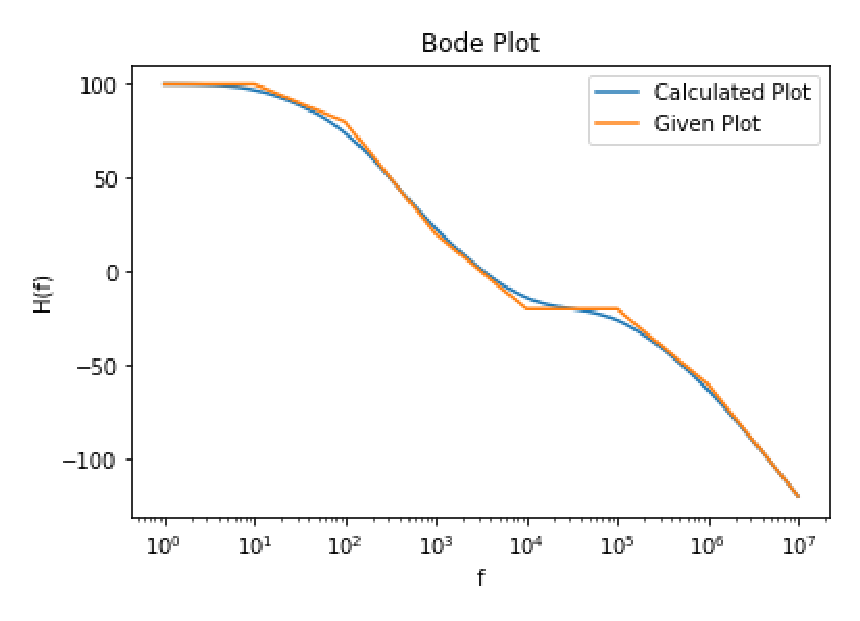
\includegraphics[width=\columnwidth]{./figs/ee18btech11001_2.eps}
    \caption{}
    \label{fig:bode}
\end{figure}
\end{enumerate}